\section{Interprocess Communication}
\subsection{Aim}
To implement programs
\begin{enumerate}
  \item for communication between a child process and its parent process with the use of Ordinary Pipes.
  \item to show IPC using Named pipes.
  \item to show IPC with the help of message queue. Here there are two processes- writer and reader.
  \item to show IPC with the help of shared memory. Here there are two processes- writer and reader.
\end{enumerate}

\subsection{Theory}
\subsubsection{Pipes}
Pipes facilitate interprocess communication by directing output of 
one process to another process. Pipe can either work by a \textbf{ordinary file} 
or by a system managed \textbf{FIFO queue}
A pipe file is created using pipe system call. It has
both write end and read end. Pipe file descriptor is an array of two elements with 
one pointing to the input end and other to the output end.

\subsubsection{Message Queues}
It is a component used for IPC, or for inter-thread communication within the same
process. It makes use of a queue for messaging – the passing of control or of content.
Message queue is a linked list of messages stored within the kernel and identified
by a message queue identifier. Every message has a positive long integer type field,
a non-negative length, and the actual data bytes (corresponding to the length), all
of which are specified to msgsnd() when the message is added to a queue. A new
queue is created or an existing queue opened by msgget(). New messages are added
to the end of a queue by msgsnd() and are fetched from the queue by msgrcv(). We
don’t have to fetch the messages in a first-in, first-out order. Instead, we can fetch
messages based on their type field.

\subsection{Shared Memory}
Shared memory is a component used in IPC, where two or more process can access
the common memory. Here, communication is done via this shared memory where
changes made by one process can be viewed by anther process. The function shmget()
is used to create and return an identifier for the shared memory segment. Before
one can use a shared memory segment, we should attach to it using the function,
shmat(). Ususally the memory address to be used is automatically chosen by the
OS. After this, we can use the memory segment for communication. When we are
done with the shared memory segment, the program should detach itself from it
using shmdt(). In order to destroy the shared memory segment, shmctl() is used.


\subsection{Algorithm}
\subsubsection{Ordinary pipe}
\begin{enumerate}
  \item Initialize pipe file descriptor
  \item Fork a child process and pass the file descriptor
  \item In child process,
  \begin{enumerate}
    \item Close read end of pipe
    \item Write a message to the write end of pipe
    \item Sleep for some time
  \end{enumerate}
  \item In parent proces,
  \begin{enumerate}
    \item Wait for child process to terminate
    \item Close the write end of pipe
    \item Read from the pipe
    \item Print the message read
  \end{enumerate}
\end{enumerate}

\subsubsection{Named Pipe}
\begin{enumerate}
  \item In user1 program,
  \begin{enumerate}
    \item Make a named pipe file description with mkfifo providing a known path
    \item Repeat,
    \begin{enumerate}
      \item Open the file in write only mode
      \item Read message from the input
      \item Print the read message
      \item Write the message to the file
      \item Close the file descriptor
      \item Open the file at path on read only mode
      \item Read message from the file descriptor 
      \item Close the file
    \end{enumerate}
  \end{enumerate}
  \item In user2 program,
  \begin{enumerate}
    \item Make a named pipe file description with mkfifo providing same path
    \item Repeat,
    \begin{enumerate}
      \item Open the file at path on read only mode
      \item Read message from the file descriptor 
      \item Print the read message
      \item Close the file
      \item Open the file in write only mode
      \item Read reply from the input
      \item Write the reply to the file
      \item Close the file descriptor
    \end{enumerate}
   
  \end{enumerate}
\end{enumerate}

\subsubsection{Message Queues}
\begin{enumerate}
  \item In writer process,
  \begin{enumerate}
    \item Create a message struct with 
      message type (long) and message body (string)
    \item Create a key using ftok
    \item Create a message id using msgget
    \item Create a message with type = 1
    \item Send message using msgsnd
  \end{enumerate}

  \item In reader process,
  \begin{enumerate}
    \item Create a message struct with 
      message type (long) and message body (string)
    \item Create a key using ftok
    \item Create a message id using msgget
    \item Recieve message using msgrcv
    \item Print the recieved message
  \end{enumerate}
\end{enumerate}

\subsubsection{Shared Memory}
\begin{enumerate}
  \item In writer process, 
  \begin{enumerate}
    \item Create a key using ftok
    \item Create a shared memory segment id using shmget
    \item Attach the message using shmat
    \item Detach from the shared memory using shmdt
  \end{enumerate}
  \item In reader process, 
  \begin{enumerate}
    \item Create a key using ftok
    \item Create a shared memory segment id using shmget
    \item Read the message using shmat
    \item Print the received message
    \item Detach from the shared memory using shmdt
    \item Delete the shared memory segment using shmctl
  \end{enumerate}
\end{enumerate}

\subsection{Source Code}
\subsubsection{Ordinary pipe}
\begin{lstlisting}[language=C]
#include <stdio.h>
#include <stdlib.h>
#include <string.h>
#include <unistd.h>
#include <sys/wait.h>
#include <sys/ipc.h>

// Child proces to write message
void child_process(
  const int *pipe_fd, const char *message, const int message_length
) {
  printf("Child process writing to pipe\n");
  close(pipe_fd[0]);
  write(pipe_fd[1], message, message_length);
  printf("Writing to pipe success\n");

  sleep(1);
  printf("Child process exiting\n");
  exit(EXIT_SUCCESS);
}

// Parent process to read message from child 
void parent_process(const int *pipe_fd, const int message_length) {
  char message[50];

  wait(NULL);

  printf("Parent process reading from pipe\n");
  close(pipe_fd[1]);
  read(pipe_fd[0], message, message_length);
  close(pipe_fd[0]);
  printf("The message read is %s\n", message);

  printf("Parent process exiting\n");
  exit(EXIT_SUCCESS);
}

int main() {
  const char message[] = "Hello world";
  
  // Pipe file descriptors
  // pipe_fd[0] for read
  // pipe_fd[1] for write
  int pipe_fd[2];

  if(pipe(pipe_fd) == -1) {
    printf("Error in creating pipe\n");
    exit(EXIT_FAILURE);
  }

  if(fork()) parent_process(pipe_fd, strlen(message));

  child_process(pipe_fd, message, strlen(message));
  
  return 0;
}
\end{lstlisting}

\begin{center}
	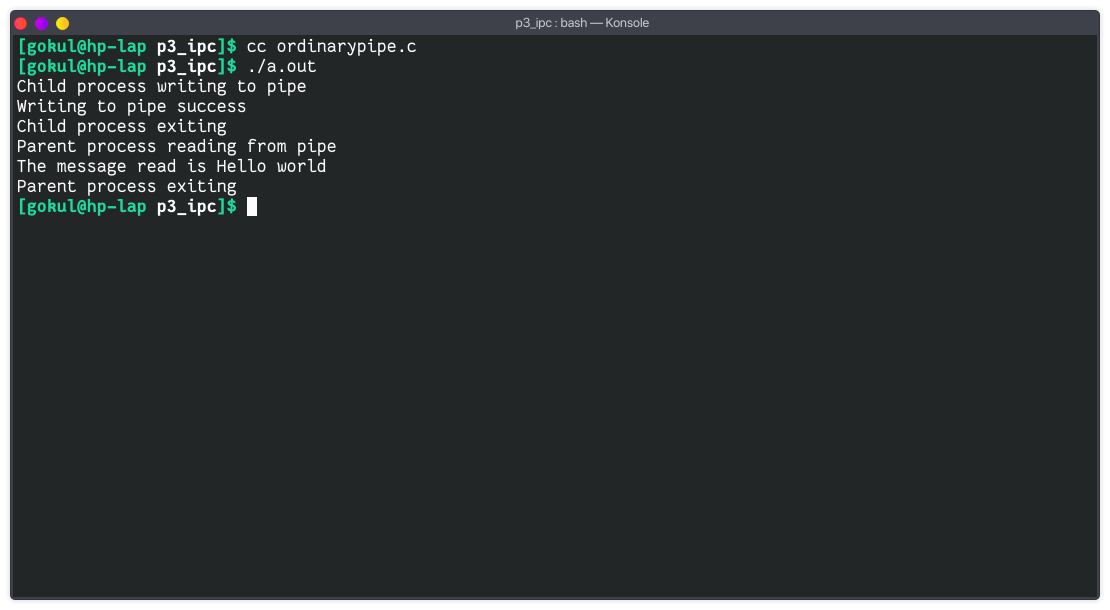
\includegraphics[width=0.90\textwidth]{img/p4/ss1.png}
\end{center}


\subsubsection{Named Pipe}
\textbf{user1.c}
\begin{lstlisting}[language=C]
#include <stdio.h>
#include <stdlib.h>
#include <unistd.h>
#include <string.h>
#include <fcntl.h>
#include <sys/types.h>
#include <sys/stat.h>

#define BUFFER_SIZE 140

int main() {
  int fd;
  const char *path = "/tmp/chat";
  char message[BUFFER_SIZE];

  mkfifo(path, 0666);

  while(1) {
    printf(">> ");
    fgets(message, BUFFER_SIZE, stdin);

    fd = open(path, O_WRONLY);
    write(fd, message, BUFFER_SIZE);
    close(fd);
    
    printf("Waiting for User2 to message\n");
    fd = open(path, O_RDONLY);
    read(fd, message, BUFFER_SIZE);
    close(fd);

    printf("User2: %s", message);
  }

  return 0;
}
\end{lstlisting}

\textbf{user2.c}
\begin{lstlisting}[language=C]
#include <stdio.h>
#include <stdlib.h>
#include <unistd.h>
#include <string.h>
#include <fcntl.h>
#include <sys/types.h>
#include <sys/stat.h>

#define BUFFER_SIZE 140

int main() {
  int fd;
  const char *path = "/tmp/chat";
  char message[BUFFER_SIZE];

  mkfifo(path, 0666);

  while(1) {
    printf("Waiting for User1 to message\n");
    fd = open(path, O_RDONLY);
    read(fd, message, BUFFER_SIZE);
    close(fd);
    
    printf("User1: %s", message);

    printf(">> ");
    fgets(message, BUFFER_SIZE, stdin);

    fd = open(path, O_WRONLY);
    write(fd, message, BUFFER_SIZE);
    close(fd);
  }

  return 0;
}  
\end{lstlisting}

\begin{center}
	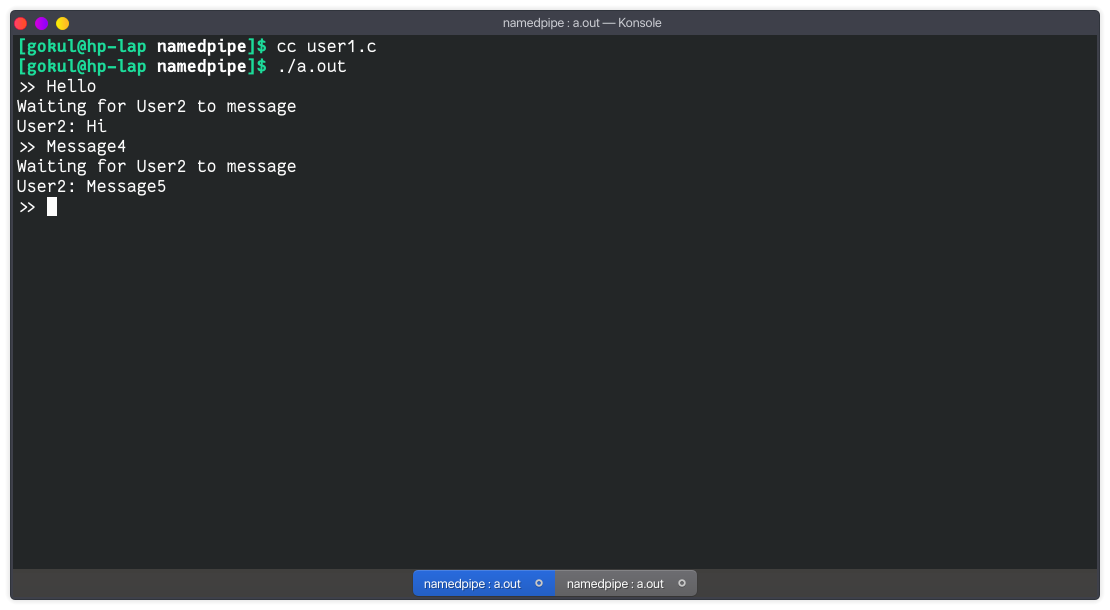
\includegraphics[width=0.90\textwidth]{img/p4/ss2.png}
	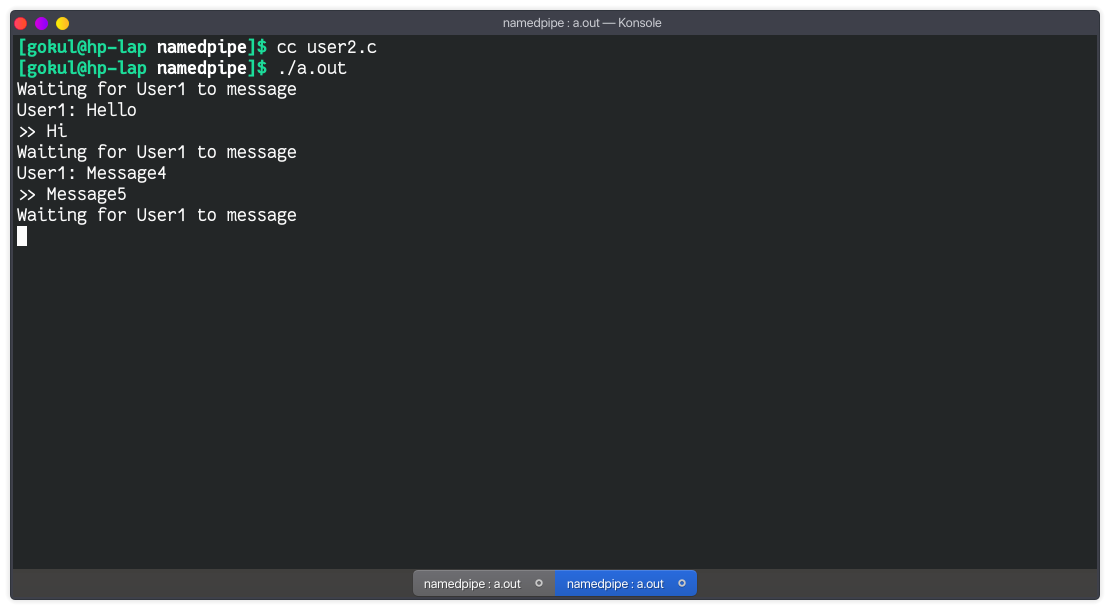
\includegraphics[width=0.90\textwidth]{img/p4/ss3.png}
\end{center}

\subsubsection{Message Queue}
\textbf{reader.c}
\begin{lstlisting}[language=C]
#include <stdio.h>
#include <stdlib.h>
#include <sys/ipc.h>
#include <sys/msg.h>

#define BUFFER_SIZE 100
#define FTOK_FILE "msgqfile"

typedef struct message {
  long type;
  char body[BUFFER_SIZE];
} message_t;

int main() {
  key_t key;
  int message_id;
  message_t message;

  key = ftok(FTOK_FILE, 'A');

  if((message_id = msgget(key, 0666 | IPC_CREAT)) < 0) {
    perror("Error getting message_id");
    exit(EXIT_FAILURE);
  }

  printf("Reading data from message queue\n");
  if(msgrcv(message_id, &message, BUFFER_SIZE, 1, 0) < 0) {
    perror("Error recieving message");
    exit(EXIT_FAILURE);
  }
  printf("Message received: %s\n", message.body);

  msgctl(message_id, IPC_RMID, NULL);

  return 0;
}
\end{lstlisting}

\textbf{writer.c}
\begin{lstlisting}[language=C]
#include <stdio.h>
#include <stdlib.h>
#include <string.h>
#include <sys/ipc.h>
#include <sys/msg.h>

#define BUFFER_SIZE 100
#define FTOK_FILE "msgqfile"

const char *messages = "Hello world";

typedef struct message {
  long type;
  char body[BUFFER_SIZE];
} message_t;

int main() {
  int message_id;
  key_t key;
  message_t message;
  int buffer_size;

  key = ftok(FTOK_FILE, 'A');

  if((message_id = msgget(key, IPC_CREAT | 0666)) < 0) {
    perror("Error getting message_id");
    exit(EXIT_FAILURE);
  }

  message.type = 1;
  strcpy(message.body, messages);
  buffer_size = strlen(message.body) + 1;

  if(msgsnd(message_id, &message, buffer_size, IPC_NOWAIT) < 0) {
    perror("Error sending message");
    exit(EXIT_FAILURE);
  }

  printf("Message sent successfully\n");
  return 0;
}
\end{lstlisting}

\begin{center}
	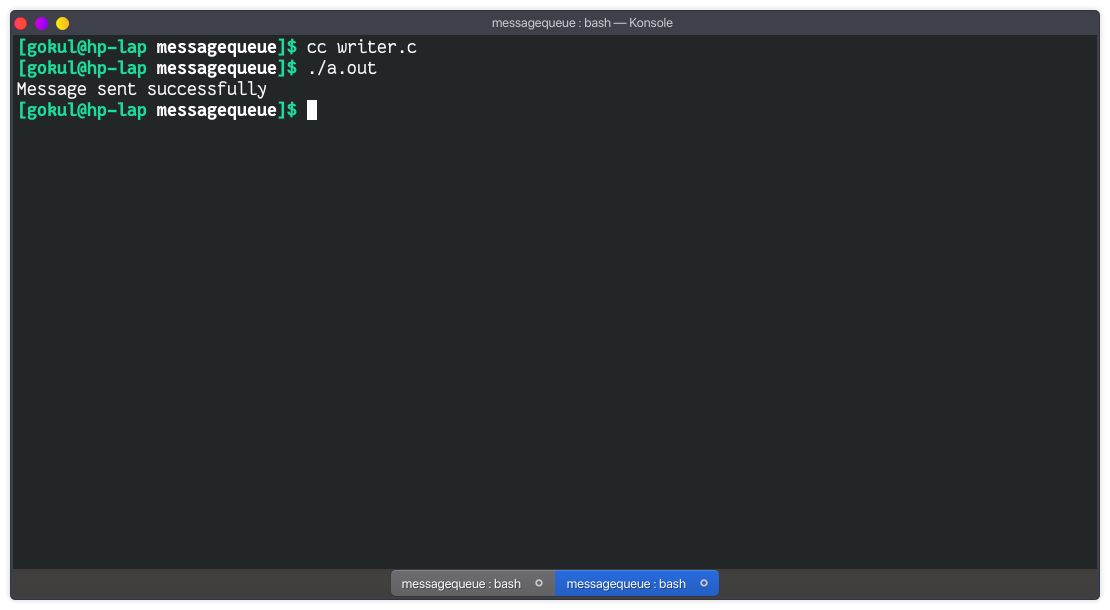
\includegraphics[width=0.90\textwidth]{img/p4/ss4.png}
	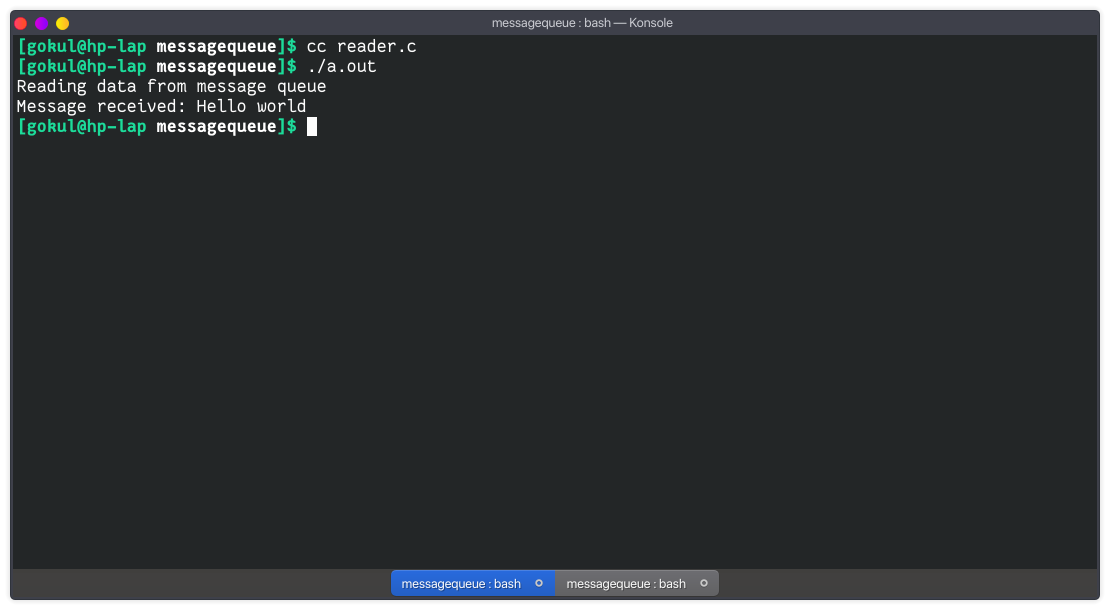
\includegraphics[width=0.90\textwidth]{img/p4/ss5.png}
\end{center}


\subsubsection{Shared Memory}
\textbf{reader.c}
\begin{lstlisting}[language=C]
#include <stdio.h>
#include <sys/msg.h>
#include <sys/shm.h>
#include <sys/ipc.h>

#define MESSAGE_LENGTH 6
#define FTOK_FILE "shmfile"

int main() {
  key_t key;
  int shm_id;
  char *message_addr;

  key = ftok(FTOK_FILE, 'A');
  shm_id = shmget(key, MESSAGE_LENGTH, 0666 | IPC_CREAT);

  printf("Reading message from shared memory segment\n");
  message_addr = (char *) shmat(shm_id, (void *)0, 0);
  printf("Message read is: %s\n", message_addr);
  shmdt(message_addr);

  shmctl(shm_id, IPC_RMID, NULL);
  return 0;
}
\end{lstlisting}

\textbf{writer.c}
\begin{lstlisting}[language=C]
#include <stdio.h>
#include <stdlib.h>
#include <string.h>
#include <sys/msg.h>
#include <sys/shm.h>
#include <sys/ipc.h>

#define MESSAGE_LENGTH 6
#define FTOK_FILE "shmfile"

int main() {
  key_t key;
  int shm_id;
  const char *message = "Hello";
  
  key = ftok(FTOK_FILE, 'A'); // Generate a unique token
  shm_id = shmget(key, MESSAGE_LENGTH, 0666 | IPC_CREAT);

  printf("Writing message to shared memory segment");
  char *message_addr = 
    (char *) shmat(shm_id, (void *)0, 0); // Attach to shared memory
  strcpy(message_addr, message);
  shmdt(message_addr); // Detach from shared memory
  printf(" SUCCESS\n");

  return 0;
}
\end{lstlisting}

\begin{center}
	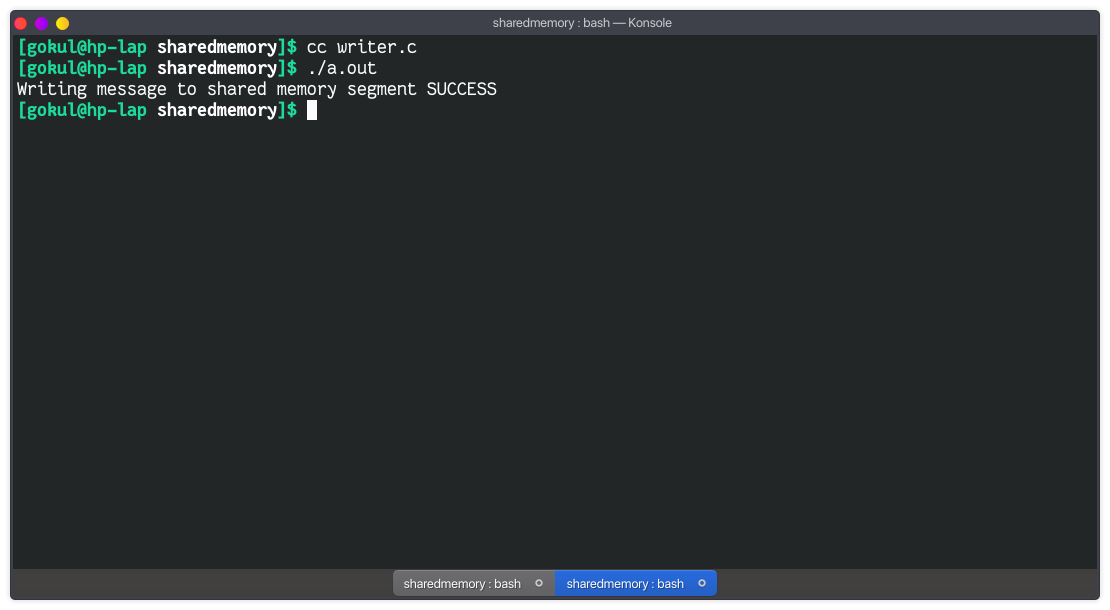
\includegraphics[width=0.90\textwidth]{img/p4/ss6.png}
	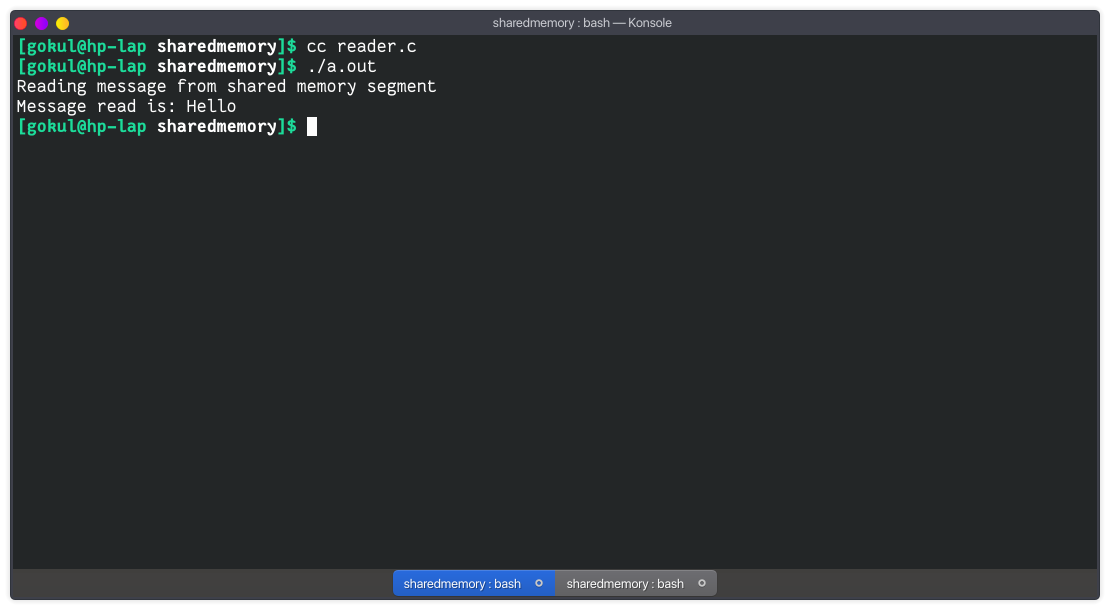
\includegraphics[width=0.90\textwidth]{img/p4/ss7.png}
\end{center}


\subsection{Result}
The above programs were executed and its output were verified